%!TEX root = ../../thesis.tex

The analysis is jet-binned because the background composition strongly depends upon jet 
multiplicity (see \Figure\todo{fig ref}). There are 0-jet and 1-jet bins, and a 
\atleast{2}-jet bin that is split into \ac{ggF} and \acsu{VBF} signal regions (see 
\Figure~\ref{fig:sig:jetbinning}). This means uncertainties should be evaluated separately 
for the exclusive bins, and correlations accounted for when the bins are combined. In the 
case of perturbative uncertainties (evaluated through scale variations), there are some 
subtleties that must be carefully considered.

\begin{figure}
	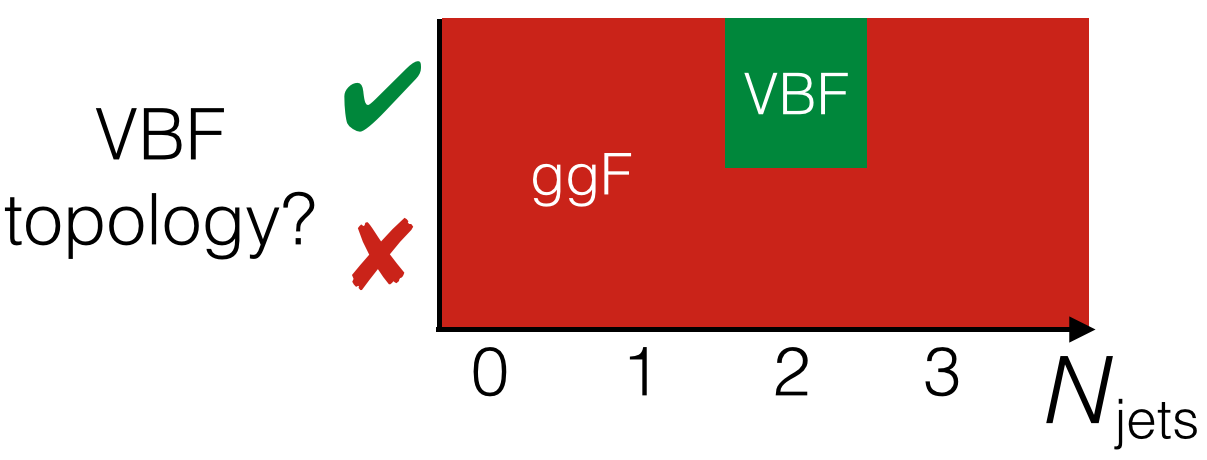
\includegraphics[width=\mediumfigwidth]{tex/signal/signal_jetbins}
	\caption{Schematic diagram of the \ac{ggF} and \ac{VBF} signal regions. Note that the 
	exclusivity of the \ac{VBF} signal region is defined by a central jet veto, and thus 
	for $\njets \geq 3$ the jet definition includes the restriction that $\eta$ is between 
	$\eta_{j_1}$ and $\eta_{j_2}$.}
	\label{fig:sig:jetbinning}
\end{figure}



\subsection{Perturbative uncertainties in exclusive jet cross sections}

Consider splitting a cross section into two parts: an exclusive $\sigma_0$ and an 
inclusive $\sigma_{\geq1}$
\begin{equation}
	\sigma_{\total} = \sigma_0 \parenths{\ptveto} + \sigma_{\geq1} \parenths{\ptveto}
\end{equation}
where \ptveto is the jet \pt threshold \cite{YR2}. The requirement of a jet with 
$\pt > \ptveto$ introduces Sudakov double logarithmic contributions 
$\alpha_{\text{S}}^{k+m} L^{2m}$ to $\sigma_{\geq1}$, where 
$L \sim \ln\parenths{\ptveto/Q}$ and $Q = \mH$ for \ac{ggF}.
These are analogous to the logarithms introduced by soft gluon emission, described in 
\Section~\ref{sec:qcd:resum}. 

The schematic structures of the two inclusive cross sections are
\begin{equation}
	\sigma_{\total} &\sim \alpha_{\text{S}}^k \{1 &+& \alphaS &+& \alpha_{\text{S}}^2 &+& \ofOrder{\alpha_{\text{S}}^3}\} \\
\sigma_{\geq1}  &\sim \alpha_{\text{S}}^k \{&\phantom{{}=+}&\alphaS (L^2 + L + 1) &+& \alpha_{\text{S}}^2 (L^4 + L^3 + L^2 + L + 1) &+& \ofOrder{\alpha_{\text{S}}^3 L^6}\}
\end{equation}
and thus the exclusive cross section is
\begin{equation}
	&\sigma_0 = \sigma_{\total} - \sigma_{\geq1} \label{eq:excl_xs_pert} \\
	&\sim \alpha_{\text{S}}^k \braces{\sqbracs{1 + \alphaS + \alpha_{\text{S}}^2 + \ofOrder{\alpha_{\text{S}}^3}} - \sqbracs{\alphaS (L^2 + L + 1) + \alpha_{\text{S}}^2 (L^4 + L^3 + L^2 + L + 1) + \ofOrder{\alpha_{\text{S}}^3 L^6}}} \,. \nonumber
\end{equation}

Corrections to $\sigma_{\total}$ are known to be large (see \Section~\ref{sec:ggf_inc}) 
and, when $\ptveto \ll \mH$, the logarithms can overcome the \alphaS suppression and 
provide significant corrections to $\sigma_{\geq1}$ too. Cancellations then occur 
between the two series in (\ref{eq:excl_xs_pert}) and the scale dependence of $\sigma_0$ 
is reduced. In fact, a \ptveto should exist such that the cancellation is exact and the 
scale uncertainty is zero. Clearly a na\"{i}ve scale variation is unsuitable.





\subsection{Combined inclusive method}
\subsection{Jet veto efficiency method}
\subsection{Comparison}
